\documentclass{article}

\usepackage{graphicx}
\usepackage{indentfirst}
\usepackage{enumitem}
\usepackage{geometry}
\usepackage{booktabs}
\usepackage{caption}
\usepackage{array}
\geometry{left=3cm, right=3cm, top=2cm, bottom=2cm}
\usepackage[colorlinks,linkcolor=blue]{hyperref}
\setlength{\parindent}{4em}
\usepackage[final]{pdfpages}

\title{\textbf{Design Document} \\ {\textbf{Command-line-based Monopoly Game}}\\ {\large PolyU COMP3211 Software Engineering Project, Fall 2024}}
\author{\large Group 24}
\date{\today}

\begin{document}

\maketitle{}

\section{Architecture Design}

\subsection{Architecture Overview}

The Model-View-Controller (MVC) architecture is adopted in the design of the Monopoly game.
The source code of the system is divided into three parts: Model, View, and Controller. 
The MVC architecture is chosen for several reasons and offers numerous advantages in this context:

\begin{itemize}
    \item \textbf{Separation of Concerns}: By dividing the application into three interconnected components, MVC allows developers to focus on one aspect of implementation at a time. This separation makes the codebase more manageable and easier to understand.
    \item \textbf{Modularity}: Each component (Model, View, Controller) can be developed, tested, and maintained independently. This modularity facilitates easier debugging and enhances the ability to extend the system with new features.
    \item \textbf{Reusability}: The Model component, which contains the core game logic and data, can be reused across different types of views (e.g., graphical user interface, command-line interface) without modification.
    \item \textbf{Scalability}: MVC architecture supports scalability by allowing the addition of new views or controllers without affecting the existing system. This is particularly useful for games like Monopoly, which may evolve over time with new rules or interfaces.
    \item \textbf{Maintainability}: The clear separation between the Model, View, and Controller makes it easier to locate and fix bugs, as well as to update the system. Changes in the user interface or business logic can be made independently.
    \item \textbf{Testability}: MVC promotes better testability by allowing unit tests to be written for each component independently. This ensures that the game logic can be thoroughly tested without the need for a user interface.
\end{itemize}

Classes in the Model package define the basic data types and relevant logic for data manipulation, including the important 
elements of the game, such as \texttt{Game}, \texttt{Player}, \texttt{Property}, \texttt{EffectType}, and \texttt{Effect}.
The Model is responsible for maintaining the state of the game and implementing the core game mechanics. It ensures that the game rules are enforced and provides methods for querying and updating the game state.

The Controller package is mainly responsible for the initialization, execution, saving, loading, continuation, and termination of the game.
It acts as an intermediary between the Model and the View, processing user inputs, invoking model updates, and updating the view accordingly.
The Controller also handles file-intensive operations such as saving and loading game states, ensuring that the game can be paused and resumed seamlessly.

The View package is responsible for the presentation layer of the game. It gathers the classes that define the data structures for implementing visual elements (\texttt{GameBoard}, \texttt{Box}, and \texttt{Brick}), and 
functions for some important system prompts (\texttt{Info}).
The View constructs the user interface and displays the current state of the game to the player. It also captures user interactions and forwards them to the Controller for processing.

For simplicity, some interfacing logic regarding data visualization is implemented directly in the Model package, and some user modifications and events are directly handled in the View package before being sent to the Model package.
However, the Controller package is responsible for most of the coordination between the Model and View packages and the overall control of the game. 
This separation of concerns ensures that the system is modular, making it easier to maintain and extend in the future.

\subsection{Architecture Diagram}

The diagram illustrating the architecture of the Monopoly game is shown in \hyperref[fig:arch]{Figure 1}.

\begin{figure}[ht]
    \centering
    \label{fig:arch}
    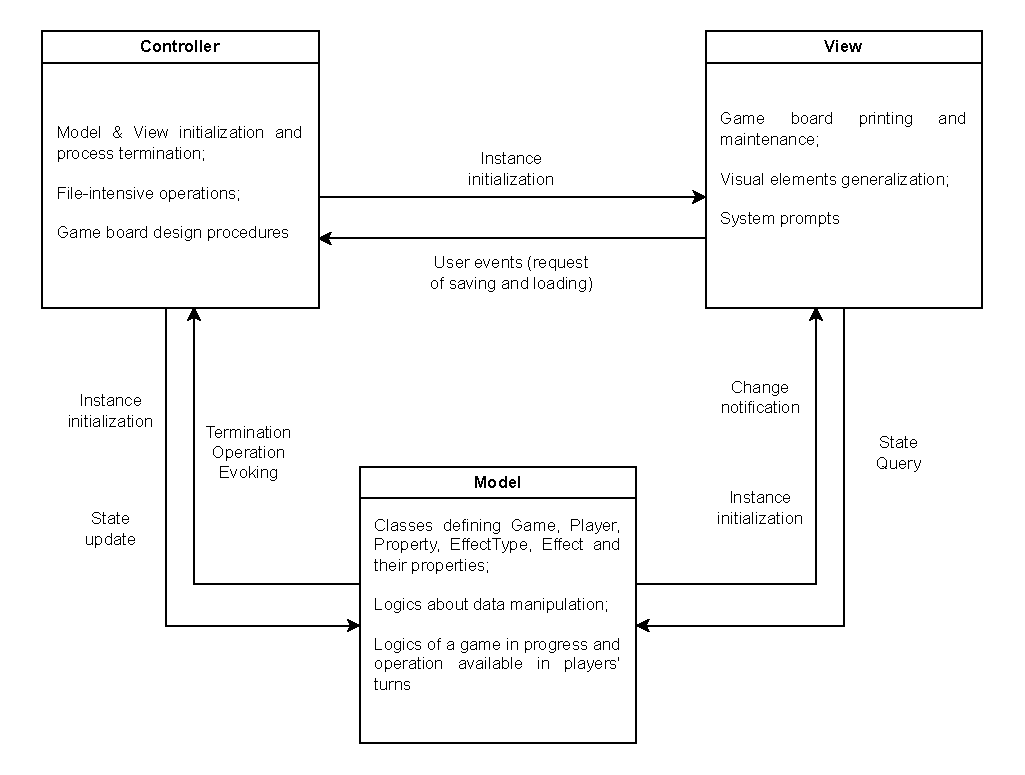
\includegraphics[width=\textwidth]{arch.drawio.pdf}
    \caption{Architecture Diagram}
\end{figure}

\section{The Structure and the Relationship among Components}

\begin{itemize}
    \item The structure and the relationship among main code components are illustrated in the class diagram on the penultimate page.
    \item The overall use cases for player and designer are shown in \hyperref[fig:playerusecase]{Figure 2} and \hyperref[fig:designerusecase]{Figure 3} respectively.
\end{itemize}

\begin{figure}[ht]
    \label{fig:playerusecase}
    \centering
    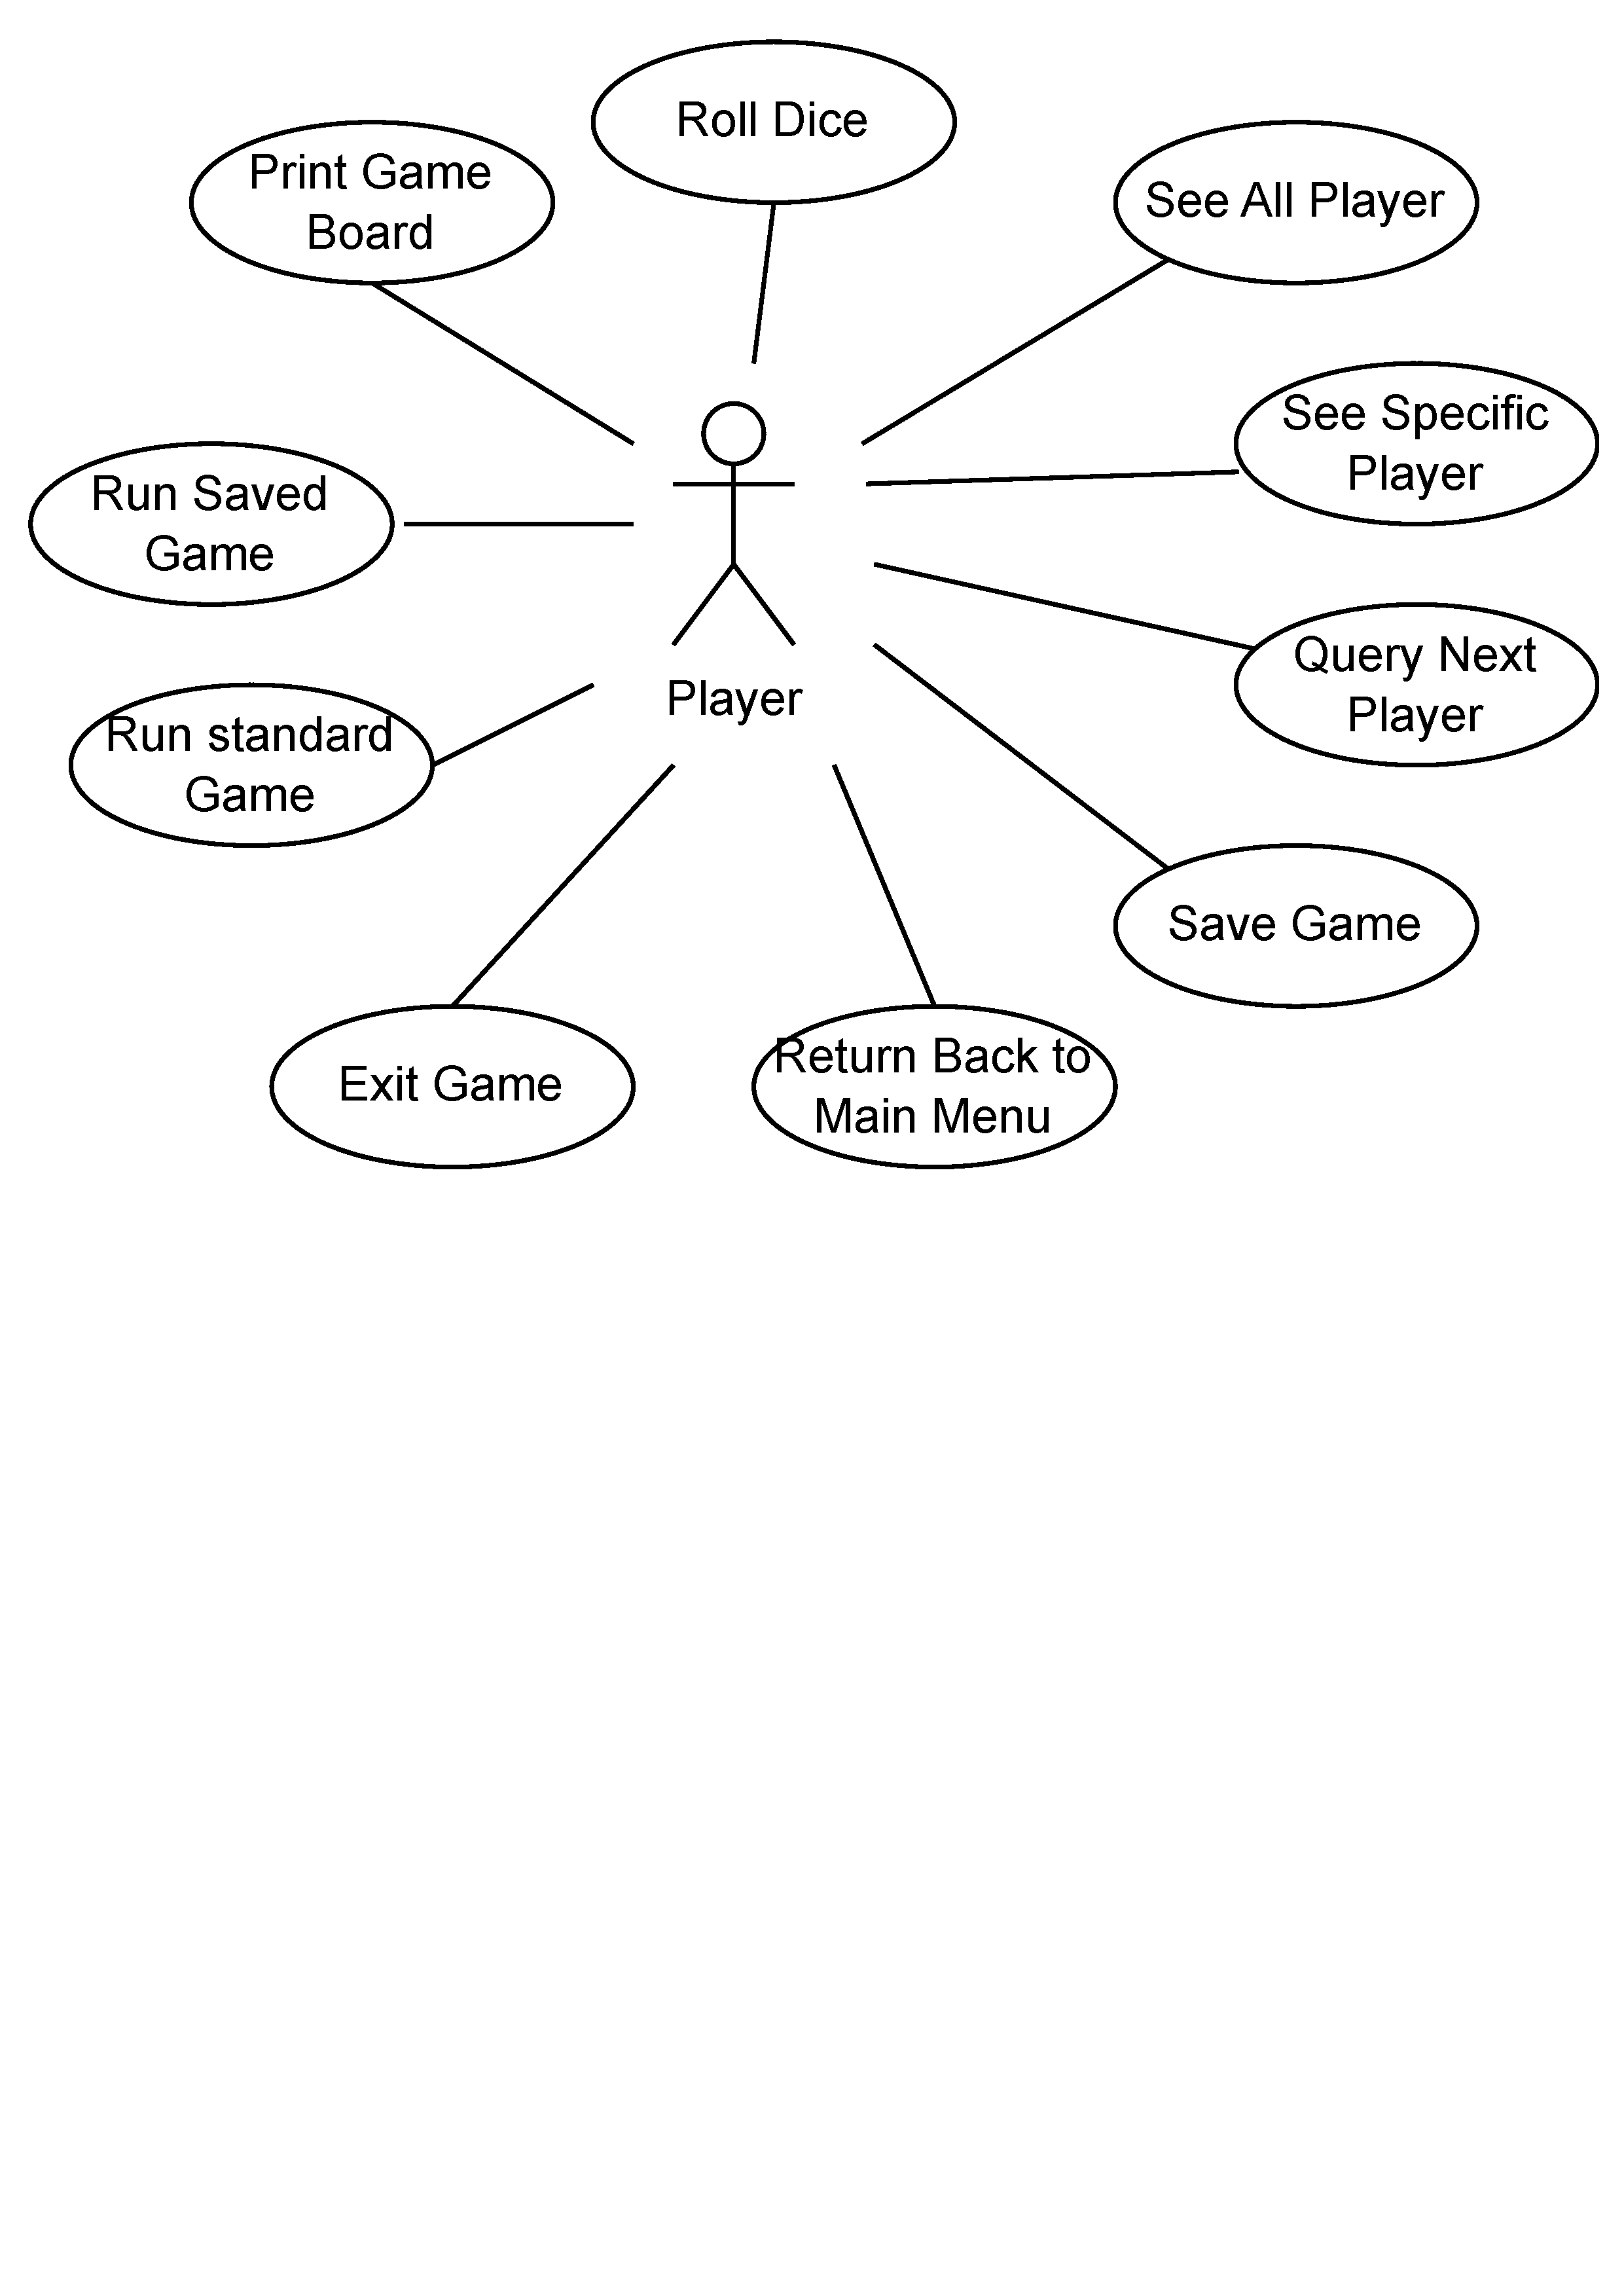
\includegraphics[width=0.8\textwidth]{crop_PlayerUseCase.drawio.pdf}
    \caption{Use Cases Diagram for Player}
\end{figure}

\begin{figure}[ht]
    \label{fig:designerusecase}
    \centering
    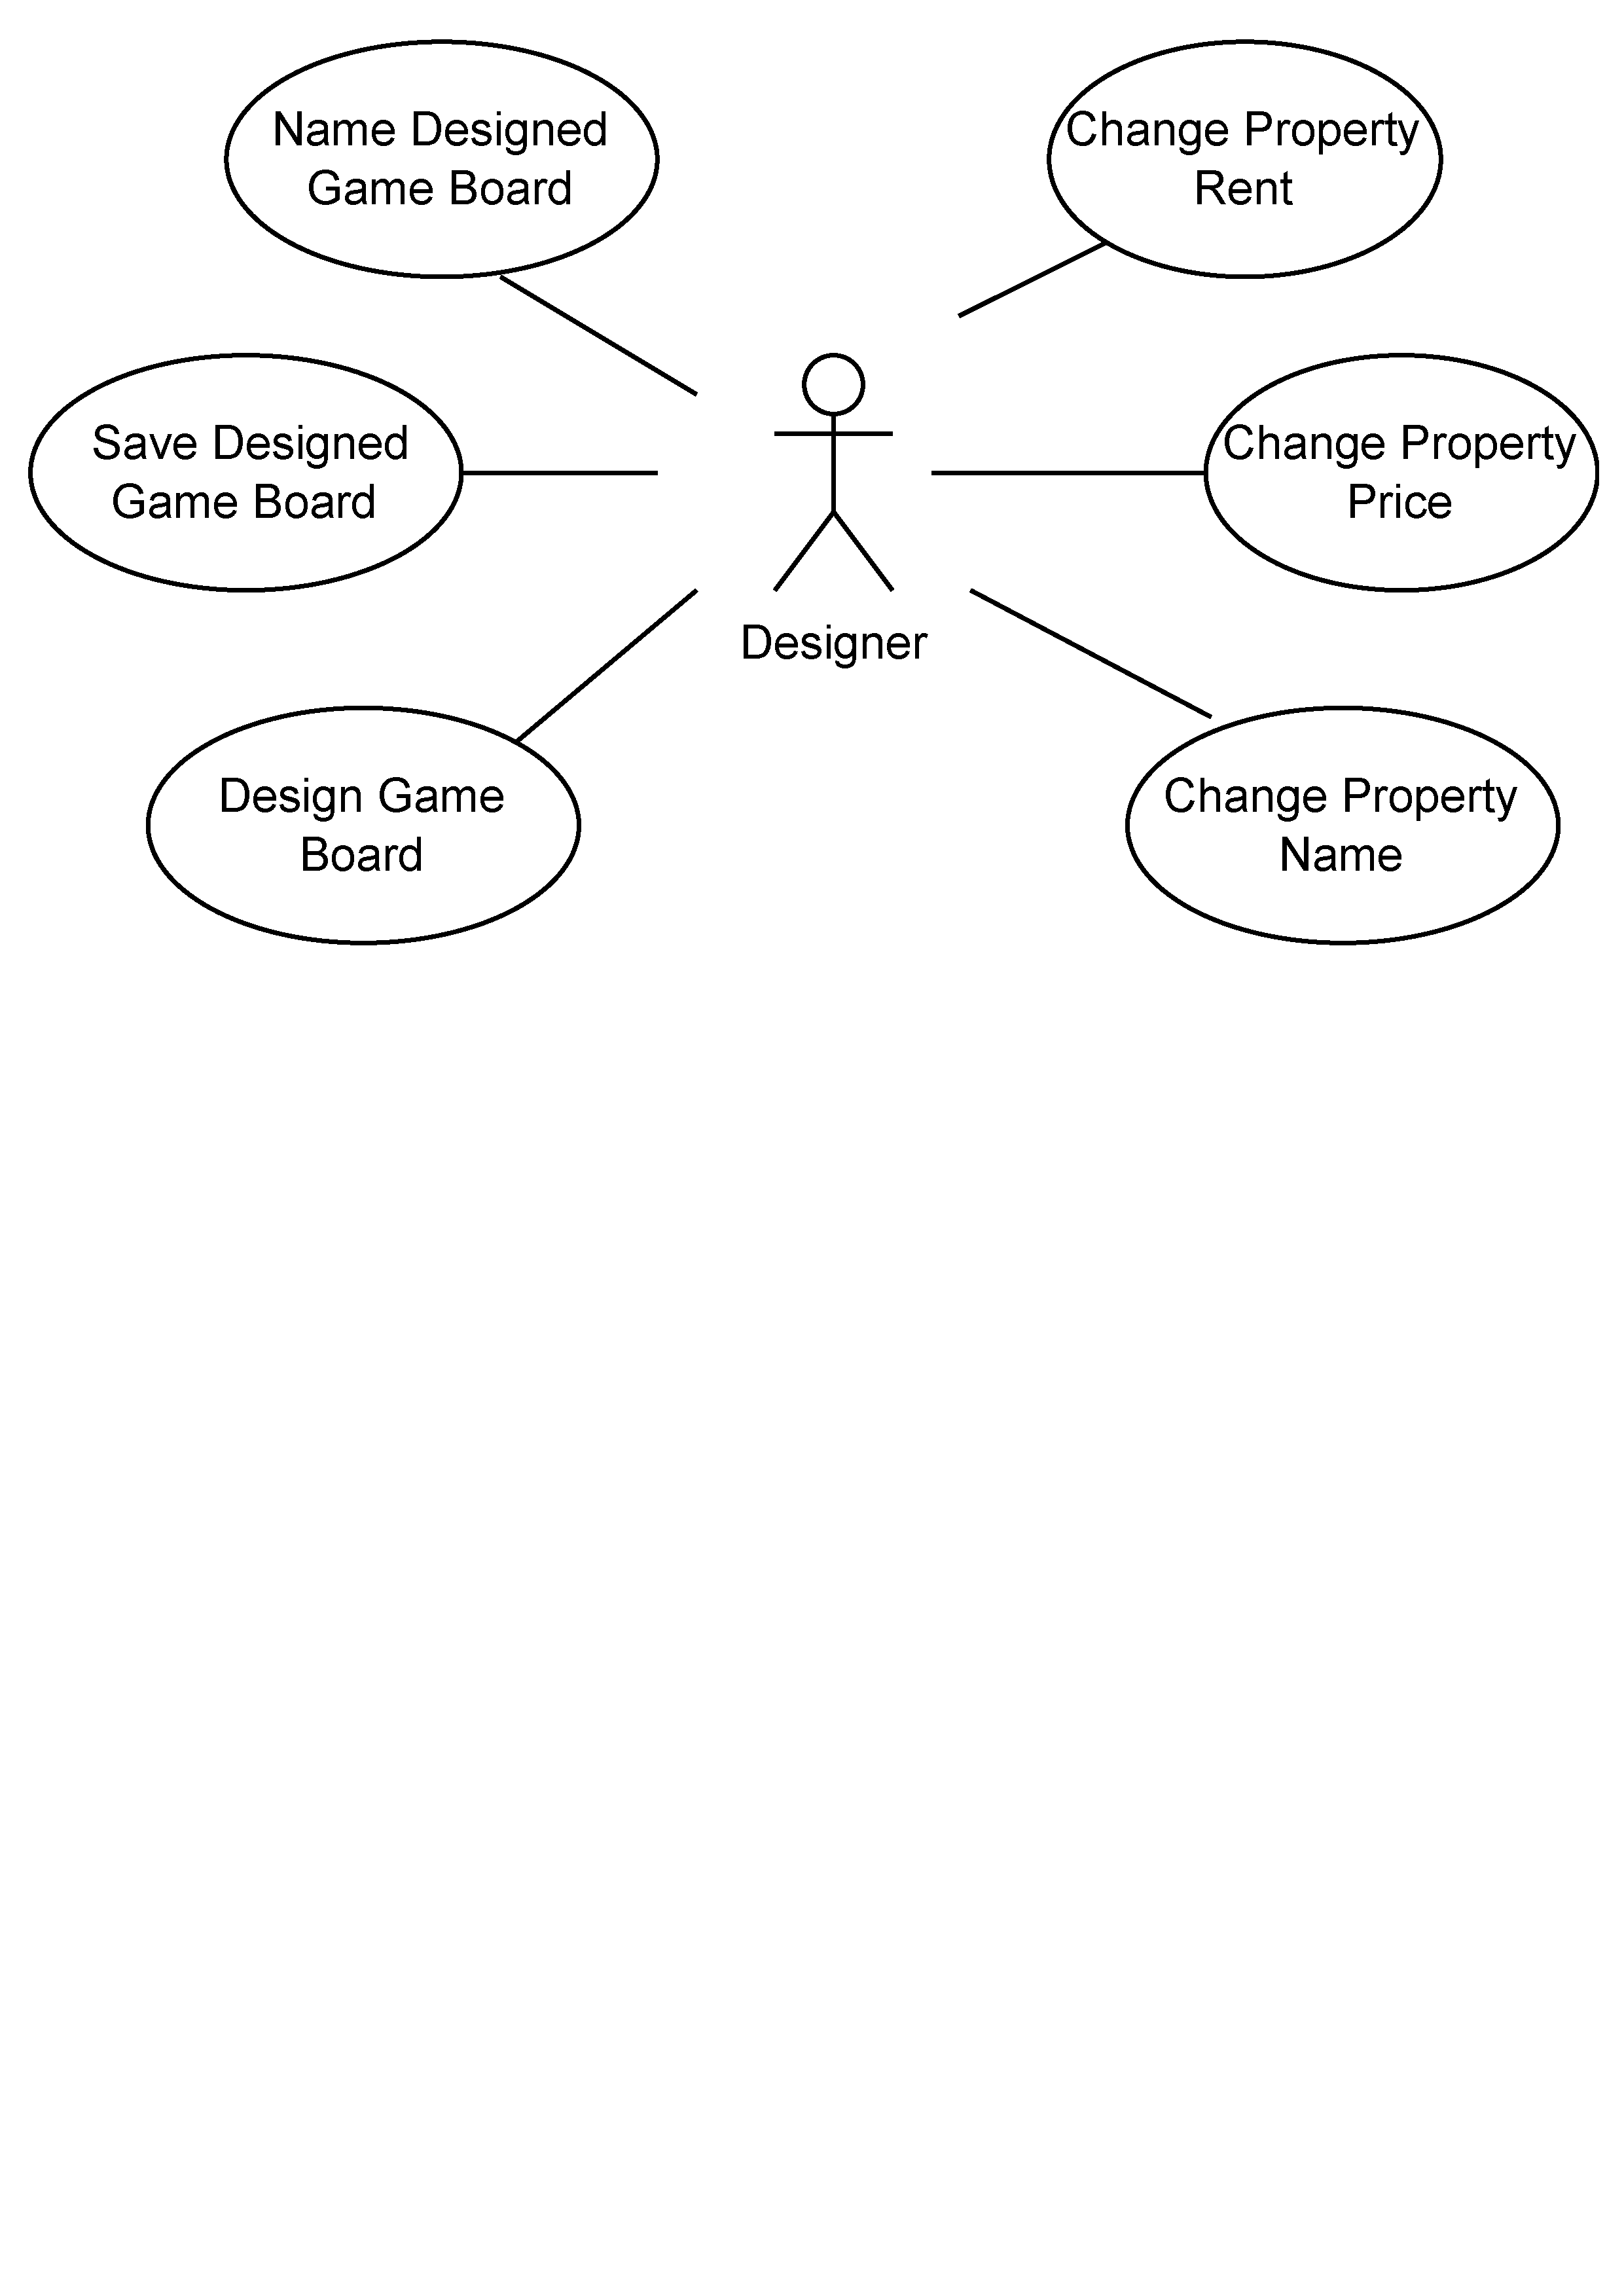
\includegraphics[width=0.8\textwidth]{crop_DesignerUseCases.drawio.pdf}
    \caption{Use Cases Diagram for Designer}
\end{figure}
\clearpage


\section{Example Use during a Turn}

The example use outlining the flow during a user's turn of playing the game is attached
in on the last page. Below is a brief summary of the sequence of events during a player's turn for the sequence diagram.

\paragraph{Lifelines}
Game System: The overarching system that manages the game flow, including player turns and game state.
Game: Represents the current game's logic, including checks for game over conditions and player actions.
Player: Represents the individual player interacting with the game system.
Sequence of Events

\paragraph{Game Loop}
The game begins with the startGame() function, which initializes the game state.
The system enters a loop that continues as long as the game is not over ([!gameOver]).

\paragraph{Game State Checks}
The checkGame() method is called to determine if the game should continue or end.
If the game is over, the flow diverges into two branches:
If gameOver is false, the game continues.
If gameOver is true, the GameOver method is invoked, prompting the end of the game.

\paragraph{Player Turn}
The playerTurn() method is called to manage the actions of the current player.
If the player is in jail (isInJail), the JailTurn() method is executed, handling the specific rules for players who cannot move freely.
If the player is not in jail, the user menu is printed for the player to make a choice.
The turnOver variable is used to control the flow, determining whether the player's turn has ended or continues.
If turnOver is false, the loop continues, allowing the player to make further choices until they decide to end their turn.

\paragraph{User Menu Interaction}
The player is presented with options (choices) through the printUserMenu() method within a loop.
Depending on the player's choice.

Choice 1: Calls the rollDiceWithPrint() method, which simulates rolling the dice and prints the result. After, triggers the positionMove(Dice, Player) method, moving the player based on the dice result. Ends the player's turn by setting turnOver=true.

Choice 2: Calls the printBoard() method and prints the current game Board. Continues the player's turn by continue setting turnOver=false and let user make further decisions on player menu.

Choice 3: Displays information about all players using the allPlayer(Info) method. Continues the player's turn by continue setting turnOver=false and let user make further decisions on player menu.

Choice 4: Allows the player to check information on a specific player via specificPlayer(Info). Continues the player's turn by continue setting turnOver=false and let user make further decisions on player menu.

Choice 5: Queries the next player’s turn with queryNextPlayer(). Continues the player's turn by continue setting turnOver=false and let user make further decisions on player menu.

Choice 6: Saves the game state using saveGame(txt.file). Continues the player's turn by continue setting turnOver=false and let user make further decisions on player menu.

Choice 7: User chooses to return back to main menu, the returnBacktoMain() function is called, the game continues, and the turnover is set to true as the turn is over. A new game is waited to be started for the user at the main menu.

Choice 8: User chooses to exit the game and sets the turnOver=true and gameOver=true so the two loops ends, and the game is exited.

If none of the choices are entered like a 9 or letters, the game system will generate an ”invalid choice, please try again” message and the call printUserMenu() method again for the player to choose.

\paragraph{Game Over Handling}
If gameOver is set to true, the game reaches a conclusion, exiting the game loop and concluding the game session.



\label{fig:strucrela}
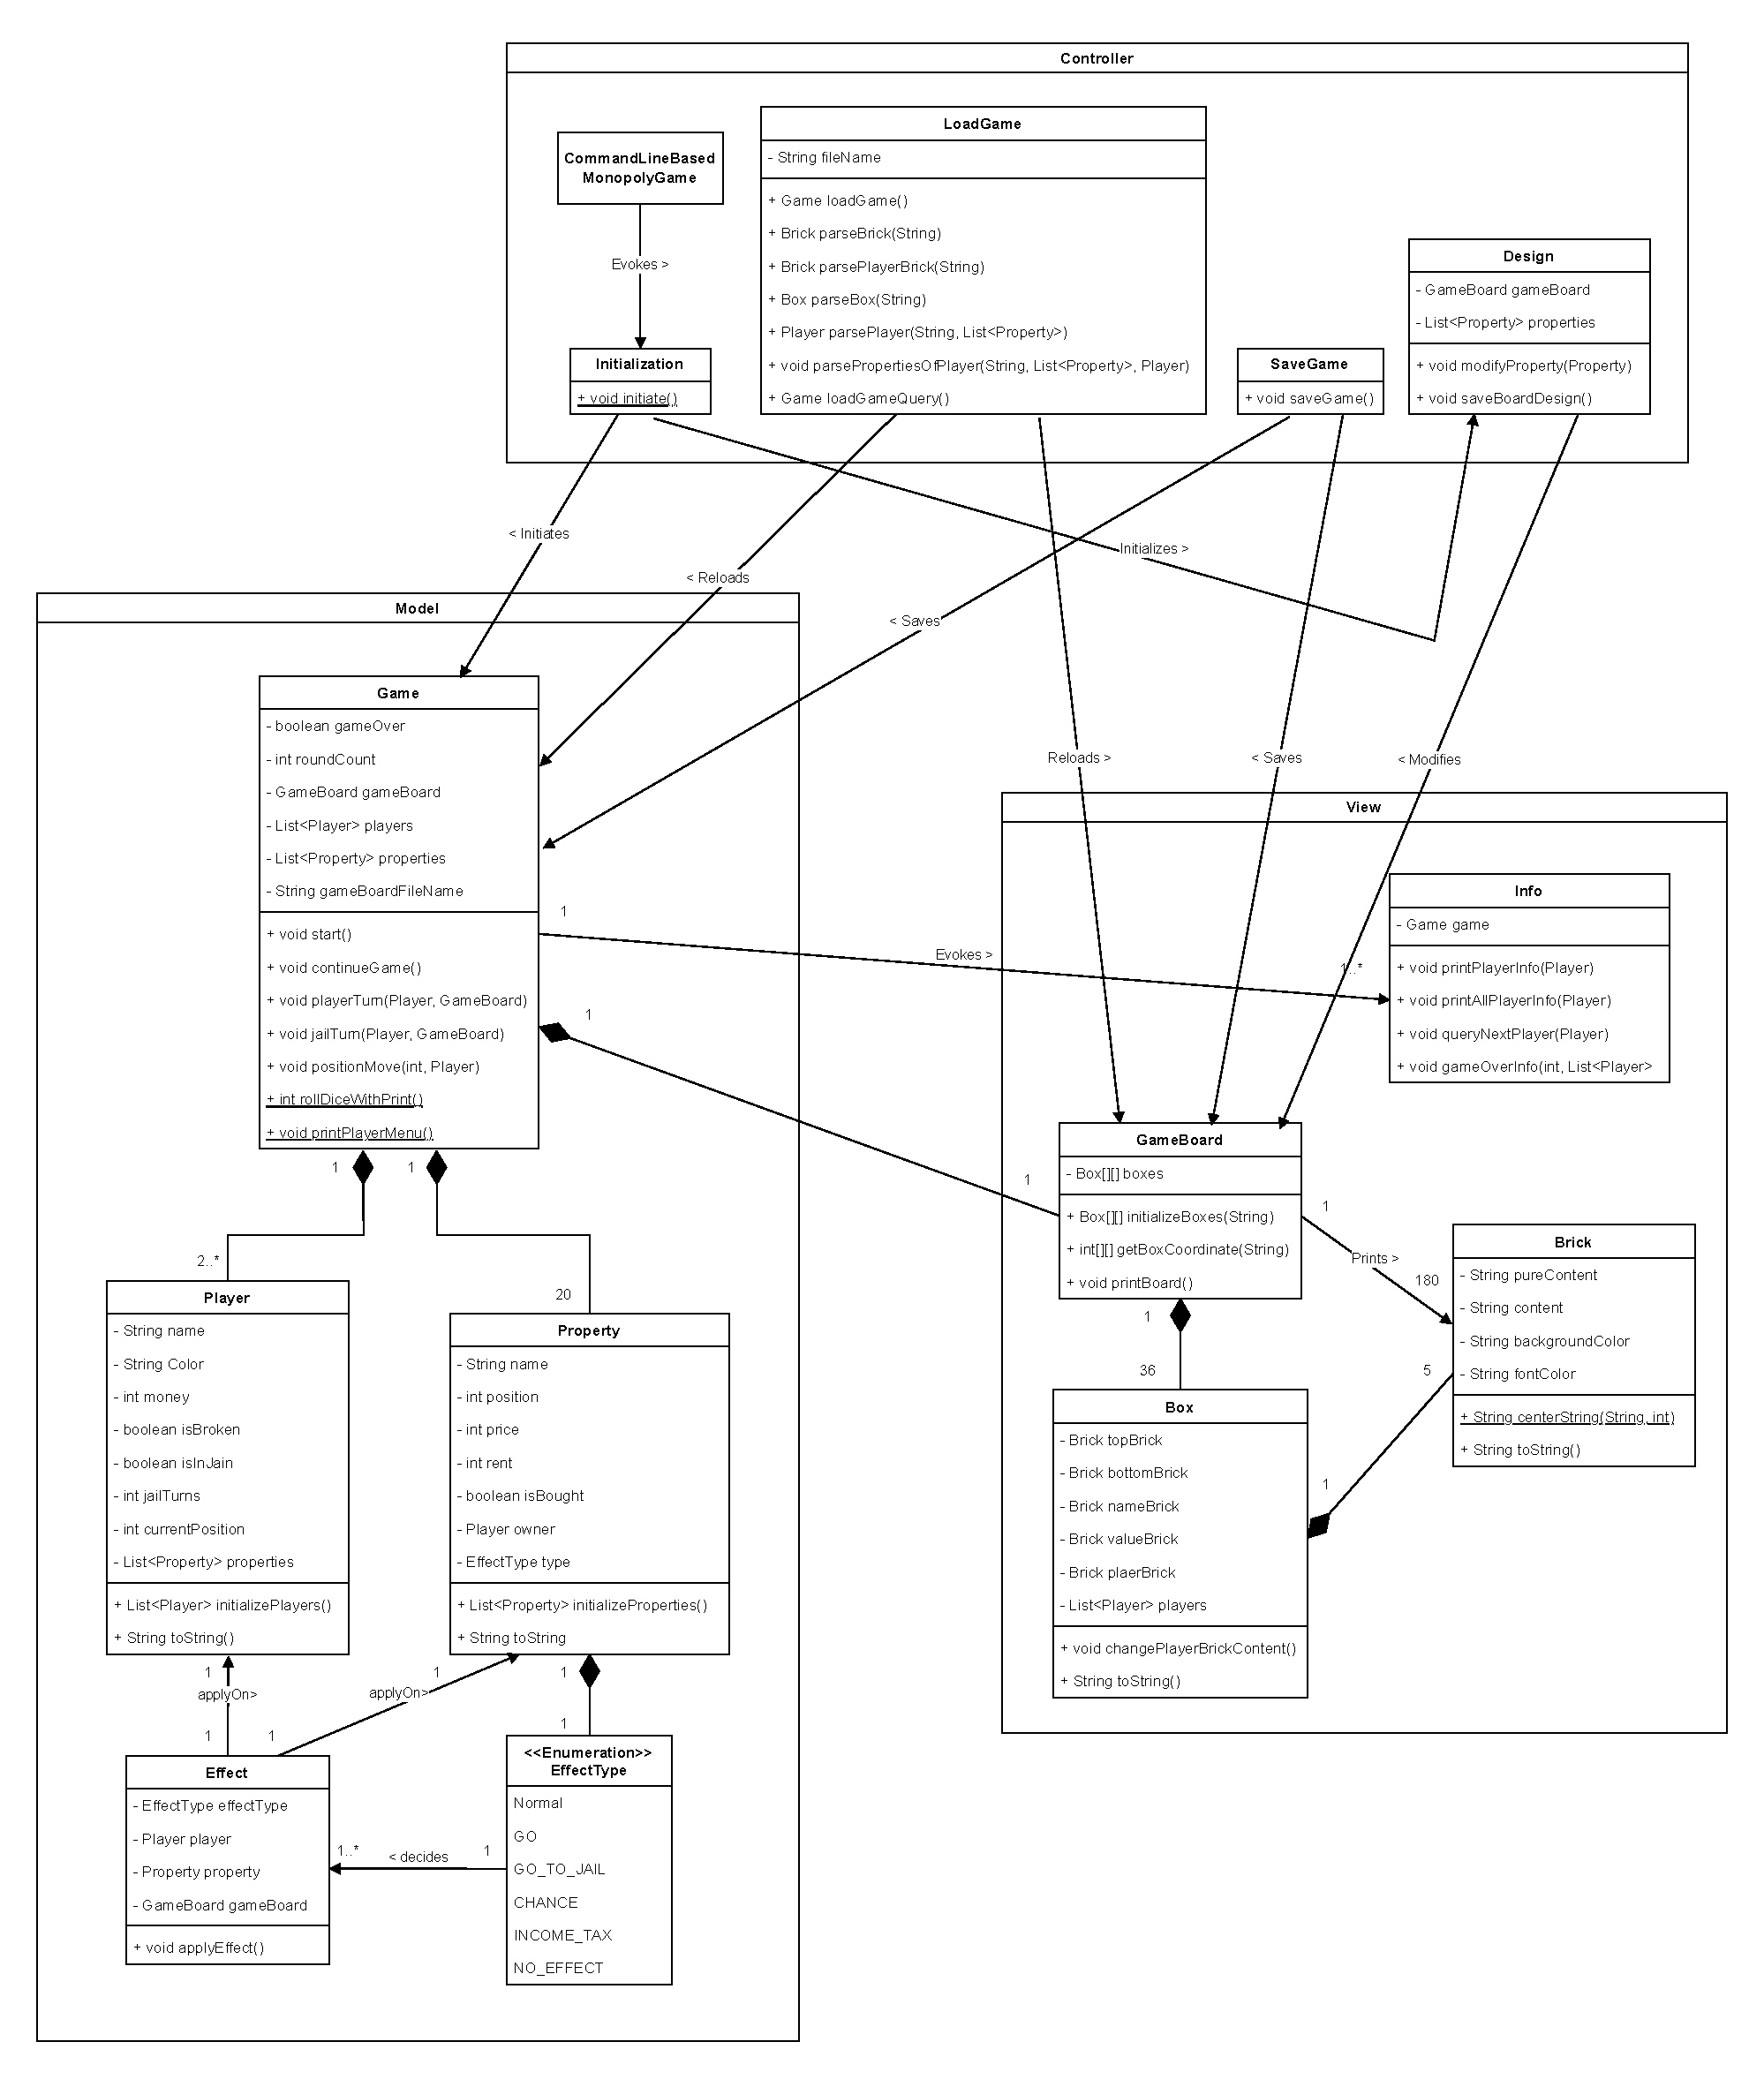
\includepdf{newnew.pdf}
\newpage

\label{fig:sequence}
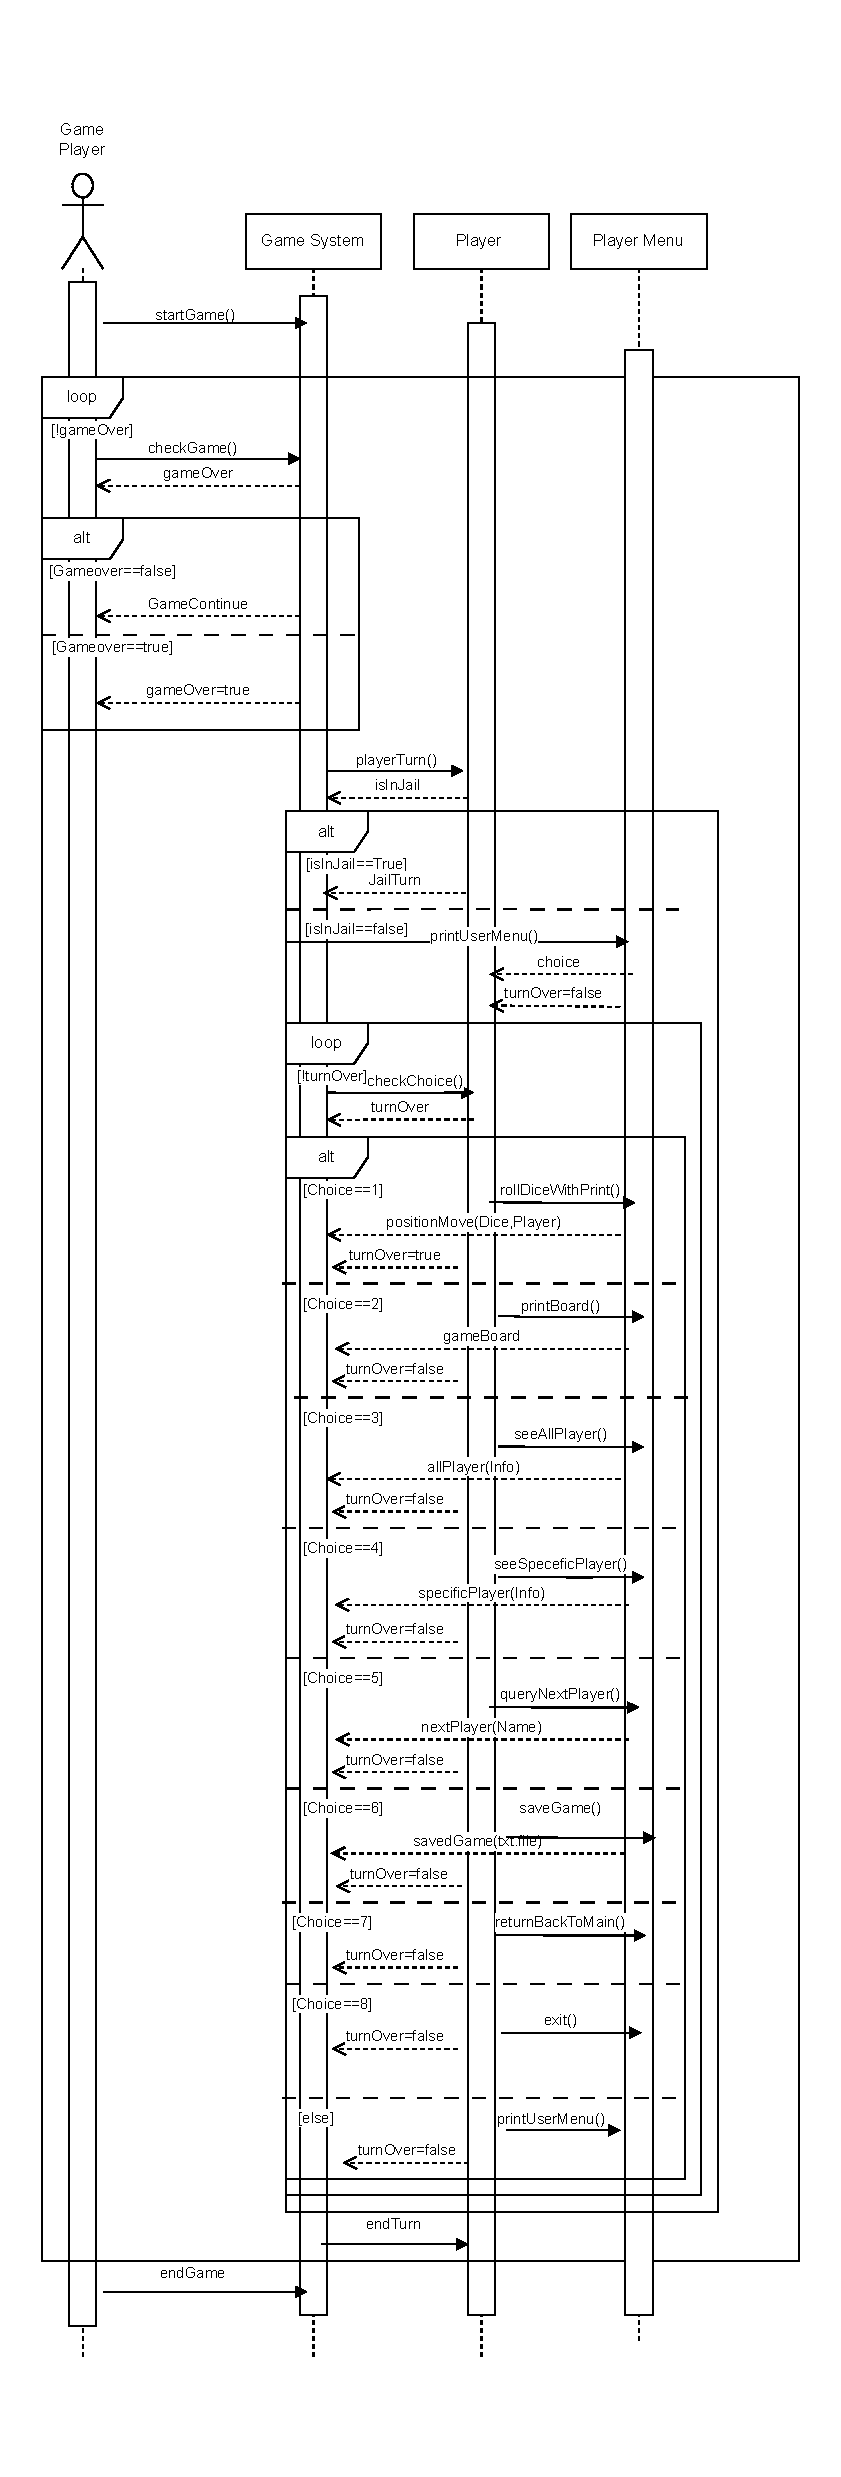
\includepdf{sequence.pdf}
\newpage

\end{document}